%*****************************************************************
%*************************** Section 7 ***************************
%**************** Streckenerkennung des Fahrzeugs ****************
%*****************************************************************


\pagestyle{fancy}
\rhead{\thepage} \chead{} \lhead{\ref{Sec7}. \nameref{Sec7}}
\cfoot{}

\section{Streckenerkennung des Fahrzeugs}\label{Sec7}

Für die Streckenerkennung des Fahrzeugs stehen zwei Kamera-Typen zur Verfügung. Zum einen kann die Pixy2 Kamera verwendet werden, welche eine Auflösung von 640x400 Bildpunkten besitzt. Die andere Möglichkeit ist eine einfache Zeilenkamera mit einer Auflösung von 1x128 Bildpunkten.\vspace{11pt}

Da in vorherigen Projekten meist die Zeilenkamera verwendet wurde, wird für dieses Projekt dieselbe eingesetzt. Ein Grund dafür ist, dass die Verwendung von Bildern von so großer Auflösung, wie bei der Pixy2 Kamera, viel Rechenressourcen und Zeit kostet. Eine geringere Auflösung ist deshalb für die Schnelligkeit des Fahrzeugs von großer Wichtigkeit. \vspace{11pt}

Da mehr als eine Kamera am Fahrzeug erlaubt ist, kann bei der Weiterführung des Projekts natürlich die Funktion einer weiteren Kamera implementiert werden. Sinnvoll kann das vor allem dann sein, wenn die additive Kamera im Gegensatz zur Zeilenkamera auf der Strecke weiter voraussieht, um Streckenverlaufs-Änderungen früher zu erkennen. Auch bei Kreuzungen, an denen die Seitenlinien kurz verschwinden, kann eine zweite Kamera dabei helfen, den Streckenverlauf nicht zu verlieren.

\subsection{Kamera des Fahrzeugs}\label{Sec7Sub1}

Wie in der Einführung dieses Kapitels bereits erwähnt, wird eine Zeilenkamera mit einer Auflösung von 1x128 Bildpunkten verwendet (TAOS TSL1401R-LF). Die Kamera kann mit einer maximalen Taktfrequenz von 8MHz betrieben werden.

\begin{figure}[H] %H für Positionierung hier
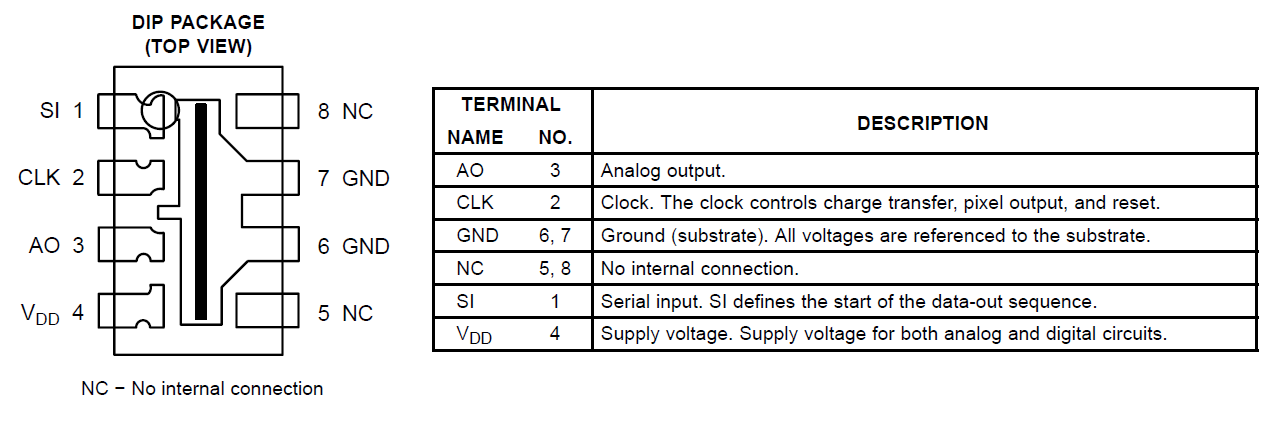
\includegraphics[width=.90\textwidth]{sec7/images/CamPinning} 
\centering
\captionsetup{width=.95\textwidth}
\caption[PinbelegungTaos Zeilenkamera TSL1401R-LF ~\protect\cite{Taos}]{Pinbelegung der Taos Zeilenkamera TSL1401R-LF ~\protect\cite{Taos}}\centering
\label{fig:CamPinning}
\end{figure}

In Abbildung \ref{fig:CamPinning} ist die Anschlussbelegung des Kamerachips und in Abbildung \ref{fig:CamWaveform} der zeitliche Verlauf einer Bildaufnahme abgebildet. Je höher die Taktfrequenz der Kamera-Clock (CLK), desto schneller kann eine Aufnahme getätigt werden. Der serielle Eingang der Kamera (SI) startet die Aufnahme. Damit die Kamera das Startsignal erkennt, muss dieses mindestens 20ns vor der steigenden Flanke der Clock anliegen (t\textsubscript{su(SI)}, \glqq{}Setup time, serial input\grqq{}). Da die \glqq{}Hold time\grqq{} des seriellen Eingangs (t\textsubscript{h(SI)}) im Datenblatt 0ns beträgt, kann sich das Rücksetzen des SI-Signals gleichzeitig mit der Clock-Flanke ereignen. Je Clock-Zyklus wird ein einzelnes Pixel ausgelesen. Die Clock-Frequenz wird deshalb von der Dauer einer ADC-Konversion beschränkt und nicht durch die technische Grenze von 8MHz.

\begin{figure}[H] %H für Positionierung hier
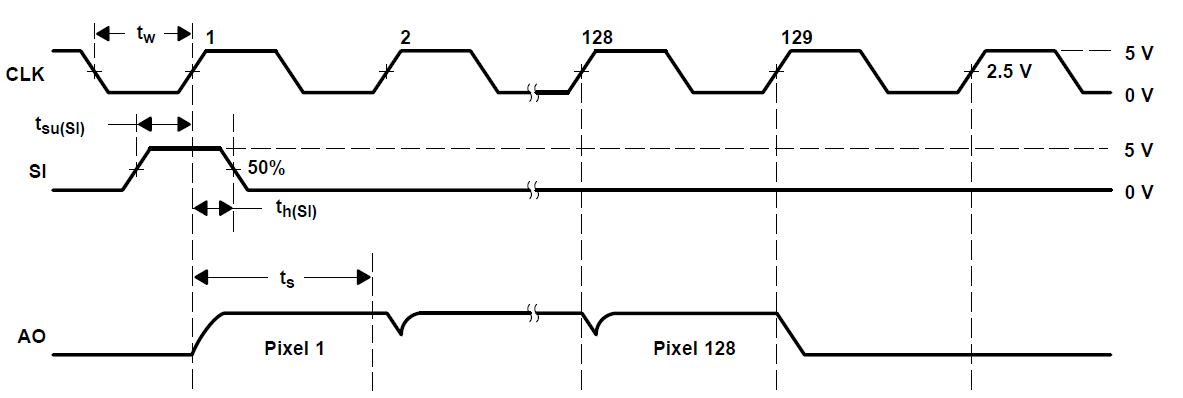
\includegraphics[width=.95\textwidth]{sec7/images/CamWaveform} 
\centering
\captionsetup{width=.95\textwidth}
\caption[Zeitverlauf einer Aufnahme mehrerer Pixel (TSL1401R-LF) ~\protect\cite{Taos}]{Zeitverlauf einer Aufnahme mehrerer Pixel mit der Kamera TSL1401R-LF ~\protect\cite{Taos}}\centering
\label{fig:CamWaveform}
\end{figure}

Nach dem 128. Clock-Zyklus ist die Aufnahme eines Bildes eigentlich abgeschlossen. Trotzdem darf die nächste Bildaufnahme erst nach 129 Clock-Zyklen und einer zusätzlichen \glqq{}Pixel Charge Transfer Time\grqq{} von 20µs erfolgen (siehe Abbildung \ref{fig:TimingWaveform}).

\begin{figure}[H] %H für Positionierung hier
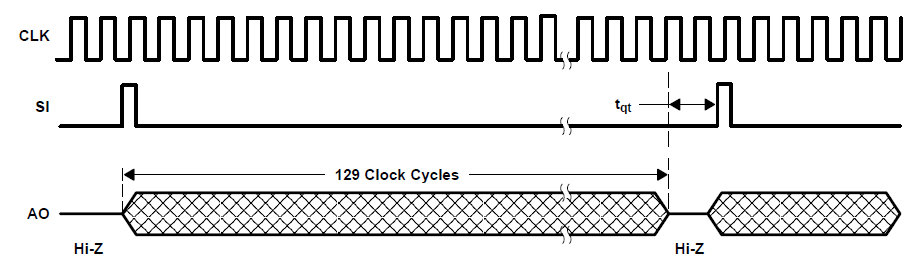
\includegraphics[width=.95\textwidth]{sec7/images/TimingWaveform} 
\centering
\captionsetup{width=.95\textwidth}
\caption[Zeitverlauf einer vollständigen Bildaufnahme (TSL1401R-LF) ~\protect\cite{Taos}]{Zeitverlauf einer vollständigen Bildaufnahme mit der Kamera TSL1401R-LF ~\protect\cite{Taos}}\centering
\label{fig:TimingWaveform}
\end{figure}

\subsection{Programmierung der Streckenauswertung}\label{Sec7Sub3}

Für die Programmierung der Streckenauswertung des Fahrzeugs werden zwei Module des Mikrocontrollers verwendet. Für die Nachbildung der zeitlichen Abläufe, die die Kamera benötigt (SI, CLK), wird der SCTimer des Controllers eingesetzt. Für diesen kann eine Vielzahl von Events konfiguriert werden. Jedes dieser Events kann andere Controller-Module triggern oder auch Ausgänge des Controllers setzen oder rücksetzen. Das zweite Modul, welches verwendet wird, ist der Analog-Digital-Wandler (ADC). Mithilfe dessen werden die Spannungspegel des analogen Ausgangs der Kamera gemessen. Diese Spannungen repräsentieren die Helligkeiten der einzelnen Pixel entsprechen.\vspace{11pt}



HIER KOMMT DIE KOMPLETTE PROGRAMMIERUNG HIN!!\vspace{11pt}


Außer der beiden verwendeten Module (ADC, SCTimer) kann es auch sinnvoll sein, den Direct Memory Access (DMA) für die Ergebnisse des ADCs und/oder einen Timer für das Triggern des seriellen Kamera-Eingangs zu verwenden. Beide Module sind in der Lage, die Bildaufnahmerate weiter zu erhöhen. Der Grund für die Erhöhung der Aufnahmerate beim Direct Memory Access ist, dass die Speicherung der Ergebnisse nach der ADC-Konversionen nicht in einer Interrupt Service Routine sondern per Direktzugriff auf den Speicher erfolgt. Die Verwendung eines Timers statt eines Tasks für das Starten einer Aufnahme, kann die Aufnahmerate ebenfalls erhöhen, da in einem Task die Wartezeit zwischen zwei Bildern durch die Funktion vTaskDelay() begrenzt ist. Diese Funktion unterstützt lediglich eine minimale Wartezeit von 1ms. Mithilfe eines Timer als Trigger kann die Wartezeit zwischen zwei Aufnahmen individualisiert und somit optimiert und verkürzt werden. Aus Zeitgründen konnten diese Funktionen allerdings nicht implementiert werden. 

\subsection{Montage und Ausrichtung der Kamera}\label{Sec7Sub2}

Für die Montage der Kamera wird die 3D-gedruckte Kamera-Halterung aus Kapitel \ref{Sec2Sub2SubSub6} verwendet. Die Halterung lässt zum einen eine individuelle Einstellung der Höhe zu und zum anderen ermöglicht die Verzahnung der Halterung eine individuelle Ausrichtung der Kamera.\vspace{11pt} 

Da bisher lediglich die Streckenauswertung und noch nicht die Regelung implementiert werden konnte, gibt es noch keine Erfahrungswerte für die optimale Positionierung und Ausrichtung der Kamera am Fahrzeug.

%\subsection{Kameralinsen}\label{Sec7Sub4}
%***CHRIS***

\newpage